%% Author: Leighton Pritchard
%% Copyright: James Hutton Institute
%% 2015-03-07: Slides for teaching at University of Dundee, 17th March 2015
%% This presentation was an invited lecture on comparative genomics and visualisation
%% for the BS32010 course.

%% UNCOMMENT FOR SLIDES
\documentclass[table]{beamer}
\mode<presentation>

%% UNCOMMENT FOR HANDOUTS
%\documentclass[handout]{beamer}
\usepackage{handoutWithNotes}
\pgfpagesuselayout{4 on 1 with notes}[a4paper,border shrink=5mm]

%% GENERIC STYLE SETTINGS BELOW
\usetheme{default}
\usepackage{listings}
\usepackage{multirow}
\usepackage{xcolor}
\usepackage{hyperref}
%\usepackage[multiple]{footmisc}

\usebackgroundtemplate{

\includegraphics[width=\paperwidth,height=\paperheight]{images/hutton_background}
}
%% PRESENTATION CONFIGURATION PARAMETERS %%%%%%%%%%%%%%%%%%%%%%%%%%%%%%%%%%%%%%%
%\titlebackgroundfile{images/hutton_title}
%\framebackgroundfile{images/hutton_background}
\definecolor{hutton_green}{HTML}{78A22F}
\definecolor{hutton_purple}{HTML}{872175}
\definecolor{hutton_blue}{HTML}{569BBE}
\definecolor{olive}{rgb}{0.3, 0.4, .1}
\definecolor{fore}{RGB}{249,242,215}
\definecolor{back}{RGB}{51,51,51}
\definecolor{title}{RGB}{255,0,90}
\definecolor{dgreen}{rgb}{0.,0.6,0.}
\definecolor{gold}{rgb}{1.,0.84,0.}
\definecolor{JungleGreen}{cmyk}{0.99,0,0.52,0}
\definecolor{BlueGreen}{cmyk}{0.85,0,0.33,0}
\definecolor{RawSienna}{cmyk}{0,0.72,1,0.45}
\definecolor{Magenta}{cmyk}{0,1,0,0}
\usefonttheme{structurebold}
\setbeamercolor{alerted text}{fg=orange}
\setbeamercolor{background canvas}{bg=white}
\setbeamercolor{block title}{bg=hutton_purple}
\setbeamercolor{frametitle}{fg=hutton_purple}
\setbeamercolor{title}{fg=black}
\setbeamercolor{titlelike}{fg=hutton_green}
\setbeamercolor{author}{fg=hutton_purple}
\setbeamercolor{author in head/foot}{fg=white}
\setbeamercolor{title in head/foot}{fg=white}
\setbeamercolor{section in head/foot}{fg=hutton_purple}
\setbeamercolor{normal text}{fg=black}
\setbeamercolor{frametitle}{fg=hutton_purple}
\setbeamerfont{block title}{size={}}
\setbeamerfont{author}{size=\footnotesize}
\setbeamerfont{institute}{size=\tiny}
\setbeamerfont{date}{size=\footnotesize}
\setbeamercolor{section in toc shaded}{fg=hutton_purple}
\setbeamercolor{section in toc}{fg=hutton_purple}
\setbeamercolor{subsection in toc shaded}{fg=hutton_purple}
\setbeamercolor{subsection in toc}{fg=hutton_purple}
\setbeamertemplate{itemize item}[circle]
\setbeamertemplate{itemize subitem}[circle]
\setbeamertemplate{itemize subsubitem}[circle]
\setbeamertemplate{itemize subsubsubitem}[circle]
\setbeamercolor{itemize item}{fg=hutton_purple}
\setbeamercolor{itemize subitem}{fg=hutton_purple}
\setbeamercolor{itemize subsubitem}{fg=hutton_purple}
\setbeamercolor{itemize subsubsubitem}{fg=hutton_purple}
\setbeamercolor{enumerate item}{fg=hutton_purple}
\setbeamercolor{enumerate subitem}{fg=hutton_purple}
\setbeamercolor{enumerate subsubitem}{fg=hutton_purple}
\setbeamercolor{enumerate subsubsubitem}{fg=hutton_purple}
\setbeamercolor{alerted text}{fg=hutton_green}
\setbeamerfont{alerted text}{series=\bfseries}
% This command makes sure that acrobat reader doesn't change the colours of the slide
% when there are figures with transparencies.
\pdfpageattr {/Group << /S /Transparency /I true /CS /DeviceRGB>>}

%Disables discrete bottom navigation bar
\beamertemplatenavigationsymbolsempty

% Modify the slide titles to avoid the corner images,
\setbeamertemplate{frametitle}
{
\vspace{0.05\textheight}
\noindent\quad\begin{minipage}[t][0.12\textheight][t]{0.85\textwidth}
\insertframetitle\par
\end{minipage}
}

% Modify title page to avoid the big logo on right
\setbeamertemplate{title page}{
    \begin{picture}(0,0)
            %This ends up on top of the default background image, rather than replacing it:
            \put(-30,-165){%
                
\includegraphics[width=\paperwidth,height=\paperheight]{images/hutton_title}
            }
            \put(0,-75){%
                \begin{minipage}[b][0.4\textheight][t]{0.75\textwidth}
                    \usebeamerfont{title}\usebeamercolor[fg]{title}{\inserttitle\par}
                    \usebeamerfont{subtitle}\usebeamercolor[fg]{subtitle}{\insertsubtitle\par}
                \end{minipage}
            }
            \put(0,-125){%
                \begin{minipage}[b][0.1\textheight][t]{\textwidth}
                    \usebeamerfont{author}\usebeamercolor[fg]{author}{\insertauthor\par}
                    \usebeamerfont{institute}\usebeamercolor[fg]{institute}{\insertinstitute\par}
                \end{minipage}
            }
    \end{picture}
}

% Make \verbatim environment tiny font
\makeatletter
\def\verbatim{\tiny\@verbatim \frenchspacing\@vobeyspaces \@xverbatim}
\makeatother

%%%%%%%%%%%%%%%%%%%%%%%%%%%%%%%%%%%%%%%%%%%%%%%%%%%%%%%%%%%%%%%%%%%%%%%%%%%%%%%%

% LISTINGS SETTING
% Settings for code listings in lstlistings

\definecolor{hutton_lightgreen}{HTML}{C8F27F}

\lstset{ %
  backgroundcolor=\color{hutton_lightgreen},   % choose the background color; you must add \usepackage{color} or \usepackage{xcolor}
  basicstyle=\tiny\ttfamily,        % the size of the fonts that are used for the code
  breakatwhitespace=false,         % sets if automatic breaks should only happen at whitespace
  breaklines=true,                 % sets automatic line breaking
  captionpos=b,                    % sets the caption-position to bottom
  commentstyle=\color{red},    % comment style
  deletekeywords={...},            % if you want to delete keywords from the given language
  escapeinside={\%*}{*)},          % if you want to add LaTeX within your code
  extendedchars=true,              % lets you use non-ASCII characters; for 8-bits encodings only, does not work with UTF-8
  frame=single,                    % adds a frame around the code
  keepspaces=true,                 % keeps spaces in text, useful for keeping indentation of code (possibly needs columns=flexible)
  keywordstyle=\color{blue},       % keyword style
%  language=Octave,                 % the language of the code
  morekeywords={*,...},            % if you want to add more keywords to the set
  numbers=left,                    % where to put the line-numbers; possible values are (none, left, right)
  numbersep=5pt,                   % how far the line-numbers are from the code
  numberstyle=\tiny\color{gray}, % the style that is used for the line-numbers
  rulecolor=\color{black},         % if not set, the frame-color may be changed on line-breaks within not-black text (e.g. comments (green here))
  showspaces=false,                % show spaces everywhere adding particular underscores; it overrides 'showstringspaces'
  showstringspaces=false,          % underline spaces within strings only
  showtabs=false,                  % show tabs within strings adding particular underscores
  stepnumber=1,                    % the step between two line-numbers. If it's 1, each line will be numbered
  stringstyle=\color{violet},     % string literal style
  tabsize=4,                       % sets default tabsize to 2 spaces
  title=\lstname                   % show the filename of files included with \lstinputlisting; also try caption instead of title
}


%%%
% TITLE PREAMBLE
\title[Comparative Genomics and Visualisation: 1.Introduction] % (optional, only for long titles)
{Comparative Genomics and \\ Visualisation \\
BS32010 \\
1.Introduction}
%\subtitle{}
\author[Pritchard] % (optional, for multiple authors)
{Leighton~Pritchard$^{1,2,3}$}
\institute[The James Hutton Institute] % (optional)
{
  $^{1}$Information and Computational Sciences,\\
  $^{2}$Centre for Human and Animal Pathogens in the Environment,\\
  $^{3}$Dundee Effector Consortium,\\
  The James Hutton Institute, Invergowrie, Dundee, Scotland, DD2 5DA
}
\date[17th March 2015] % (optional)
{17th March 2015}
\subject{Bioinformatics, Genomics, Bacteria, Sequencing, Microbiology, Microbes, Comparative Genomics, Visualisation}

%%%
% TOC
% Show table of contents, with current section highlighted,
% at the start of each section

%\AtBeginSection[]
%{
%  \begin{frame}
%    \frametitle{Table of Contents}
%    \tableofcontents[currentsection] %,hideallsubsections]
%  \end{frame}
%}

\AtBeginSubsection[]
{
  \begin{frame}
    \frametitle{Table of Contents}
    \tableofcontents[currentsection,currentsubsection] %,hideallsubsections]
  \end{frame}
}

%%%
% START DOCUMENT
\begin{document}

\frame[plain]{\titlepage}

%% use.tex
%% Author: Leighton Pritchard
%% Copyright: James Hutton Institute
%% These slides describe the acceptable use policy for these slides and
%% materials

%
\begin{frame}
  \frametitle{Acceptable Use Policy}
  Recording of this talk, taking photos, discussing the content using \\
  email, Twitter, blogs, etc. is permitted (and encouraged), \\
  providing distraction to others is minimised. \\[0.5cm]
  These slides will be made available on SlideShare. \\[0.5cm]
  \textbf{These slides, and supporting material including exercises, are available at \href{https://github.com/widdowquinn/Teaching-2015-03-17-UoD_compgenvis}{https://github.com/widdowquinn/Teaching-2015-03-17-UoD\_compgenvis}}
\end{frame}

%%%
% SECTION: Introduction
\section{Introduction}

% SUBSECTION
% What is Comparative Genomics?
\subsection{What is comparative genomics?}
%% what_is_compgen.tex
%% Author: Leighton Pritchard
%% Copyright: James Hutton Institute
%% Introductory slides: What is Comparative Genomics?





%
\begin{frame}
  \frametitle{What Is Comparative Genomics?}
  \Large{
    \textcolor{olive}{
      \textbf{
      The combination of genomic data, and comparative and evolutionary biology, to address questions of   genome structure, evolution, and function.
      }
    }
  }
\end{frame}

%
\begin{frame}
  \frametitle{Evolution is the central concept}
  \begin{center}
    
\includegraphics[width=\textwidth]{images/dobzhansky_quote}
  \end{center}  
\end{frame}

%
\begin{frame}
  \frametitle{Comparison of physical features}
  How do we determine that features are related, and evolved? \\
  \begin{center}
    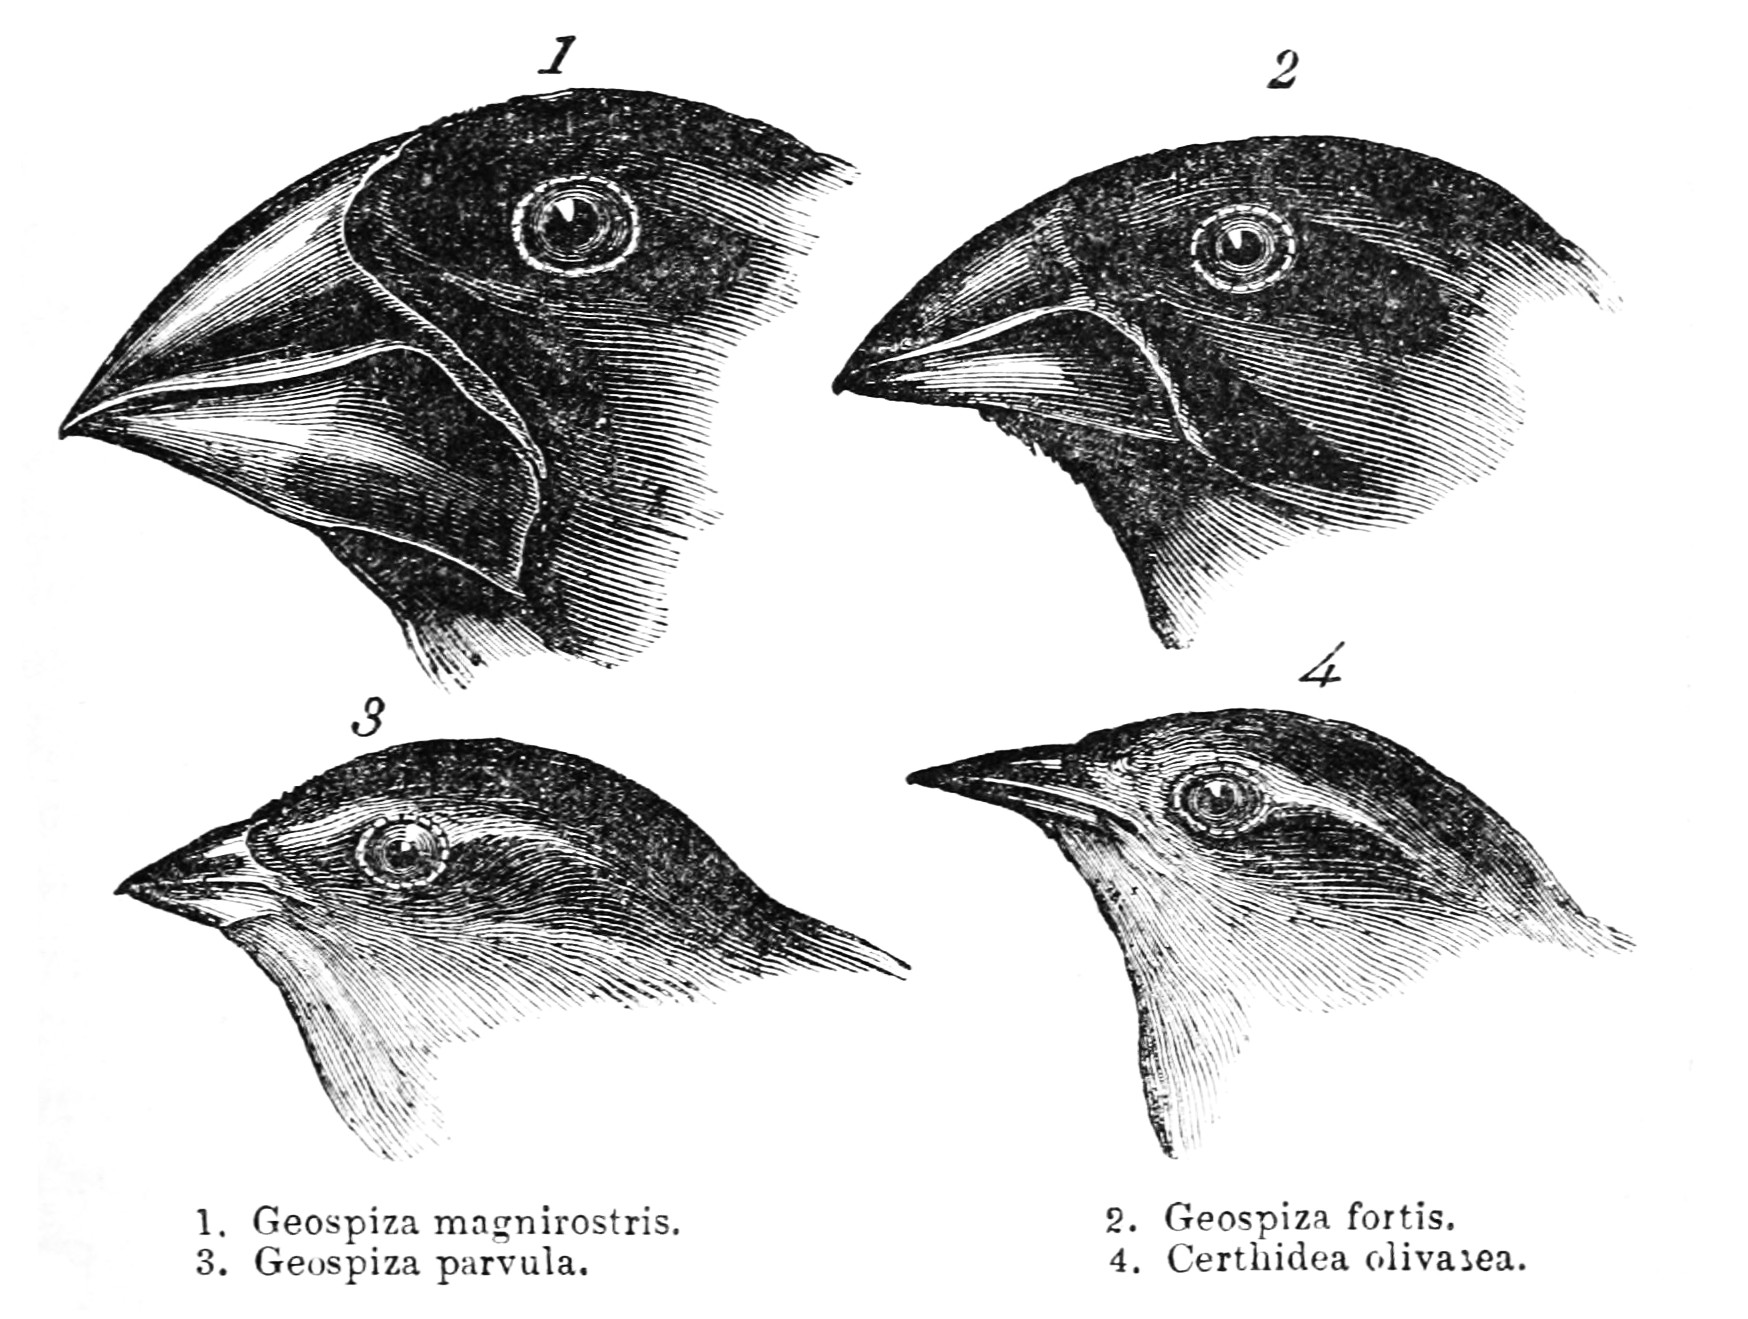
\includegraphics[width=0.8\textwidth]{images/darwin_finches}
  \end{center}  
\end{frame}

%
\begin{frame}
  \frametitle{Comparison of sequence features}
  Multiple sequence alignment of ATP synthase \\
  \begin{center}
    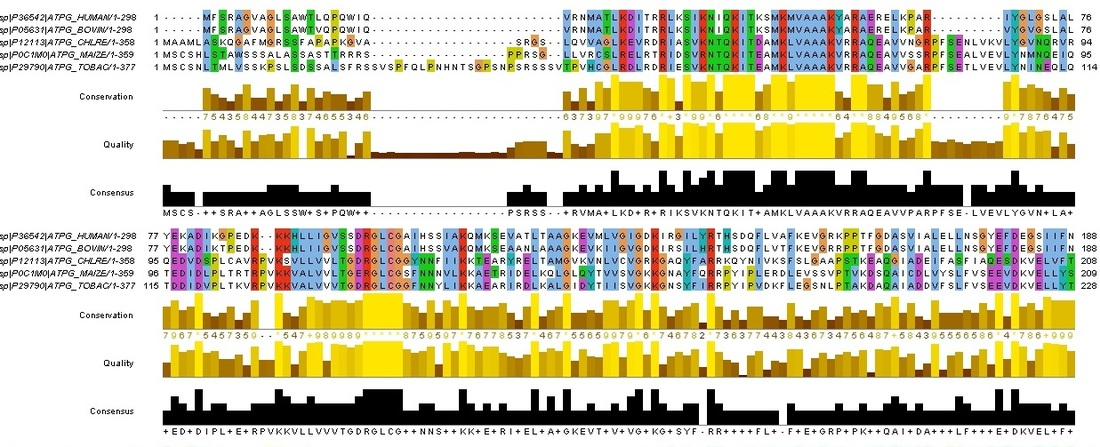
\includegraphics[width=\textwidth]{images/atp_synthase_alignment}
  \end{center}  
\end{frame}

%
\begin{frame}
  \frametitle{Comparison of genome features}
  Similarity of individual features (feature sequence) \\
  \begin{center}
    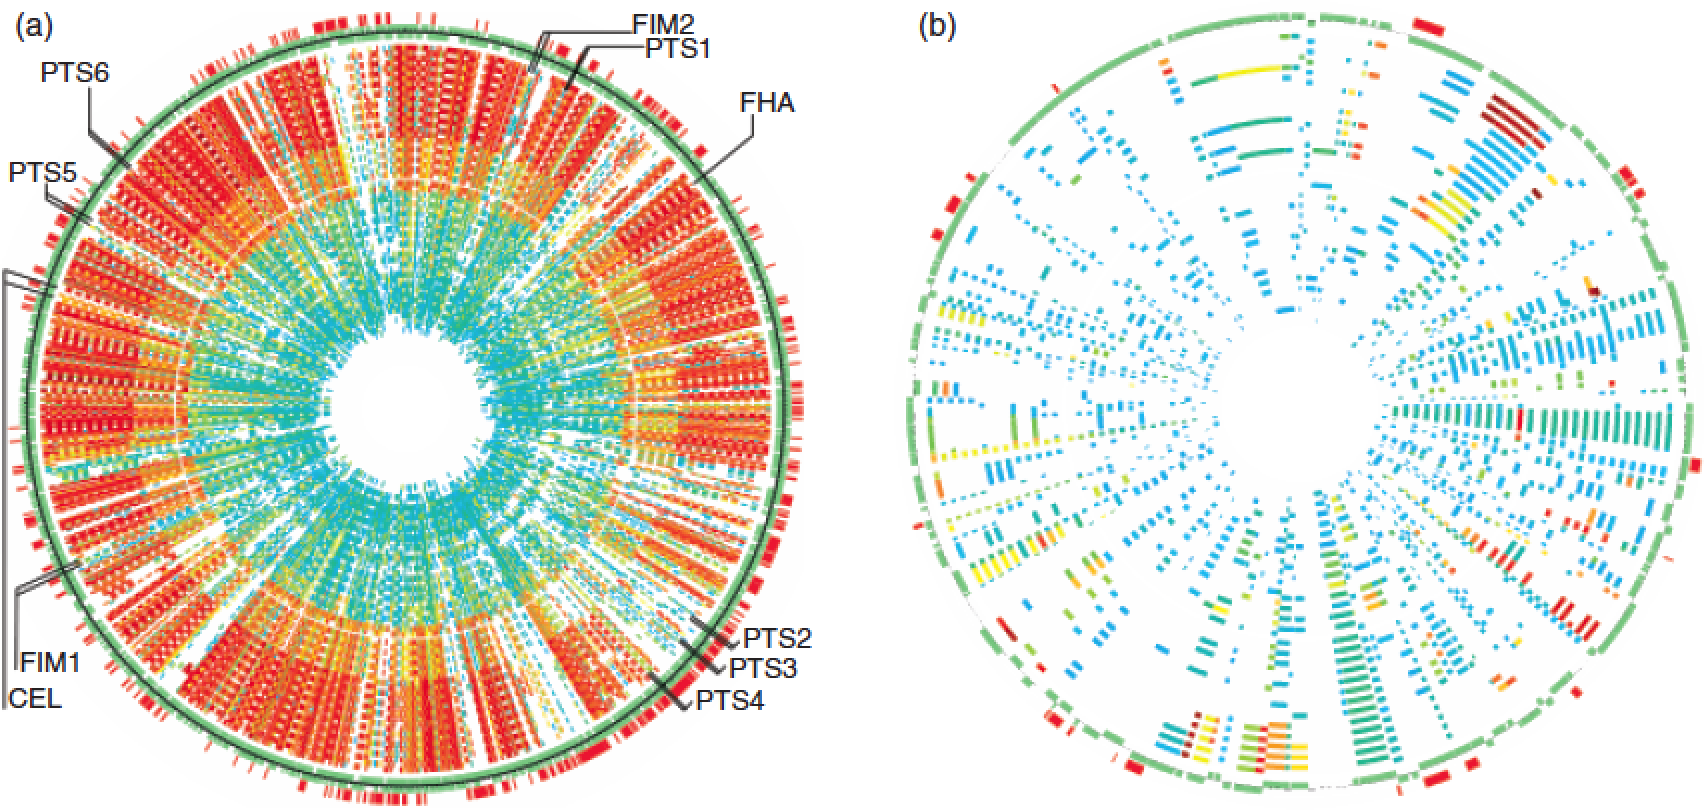
\includegraphics[width=\textwidth]{images/salmonella_circular_comparison}
  \end{center}  
\end{frame}

%
\begin{frame}
  \frametitle{Comparison of genome features}
  Similarity of individual features (ordering and arrangement) \\
  \begin{center}
    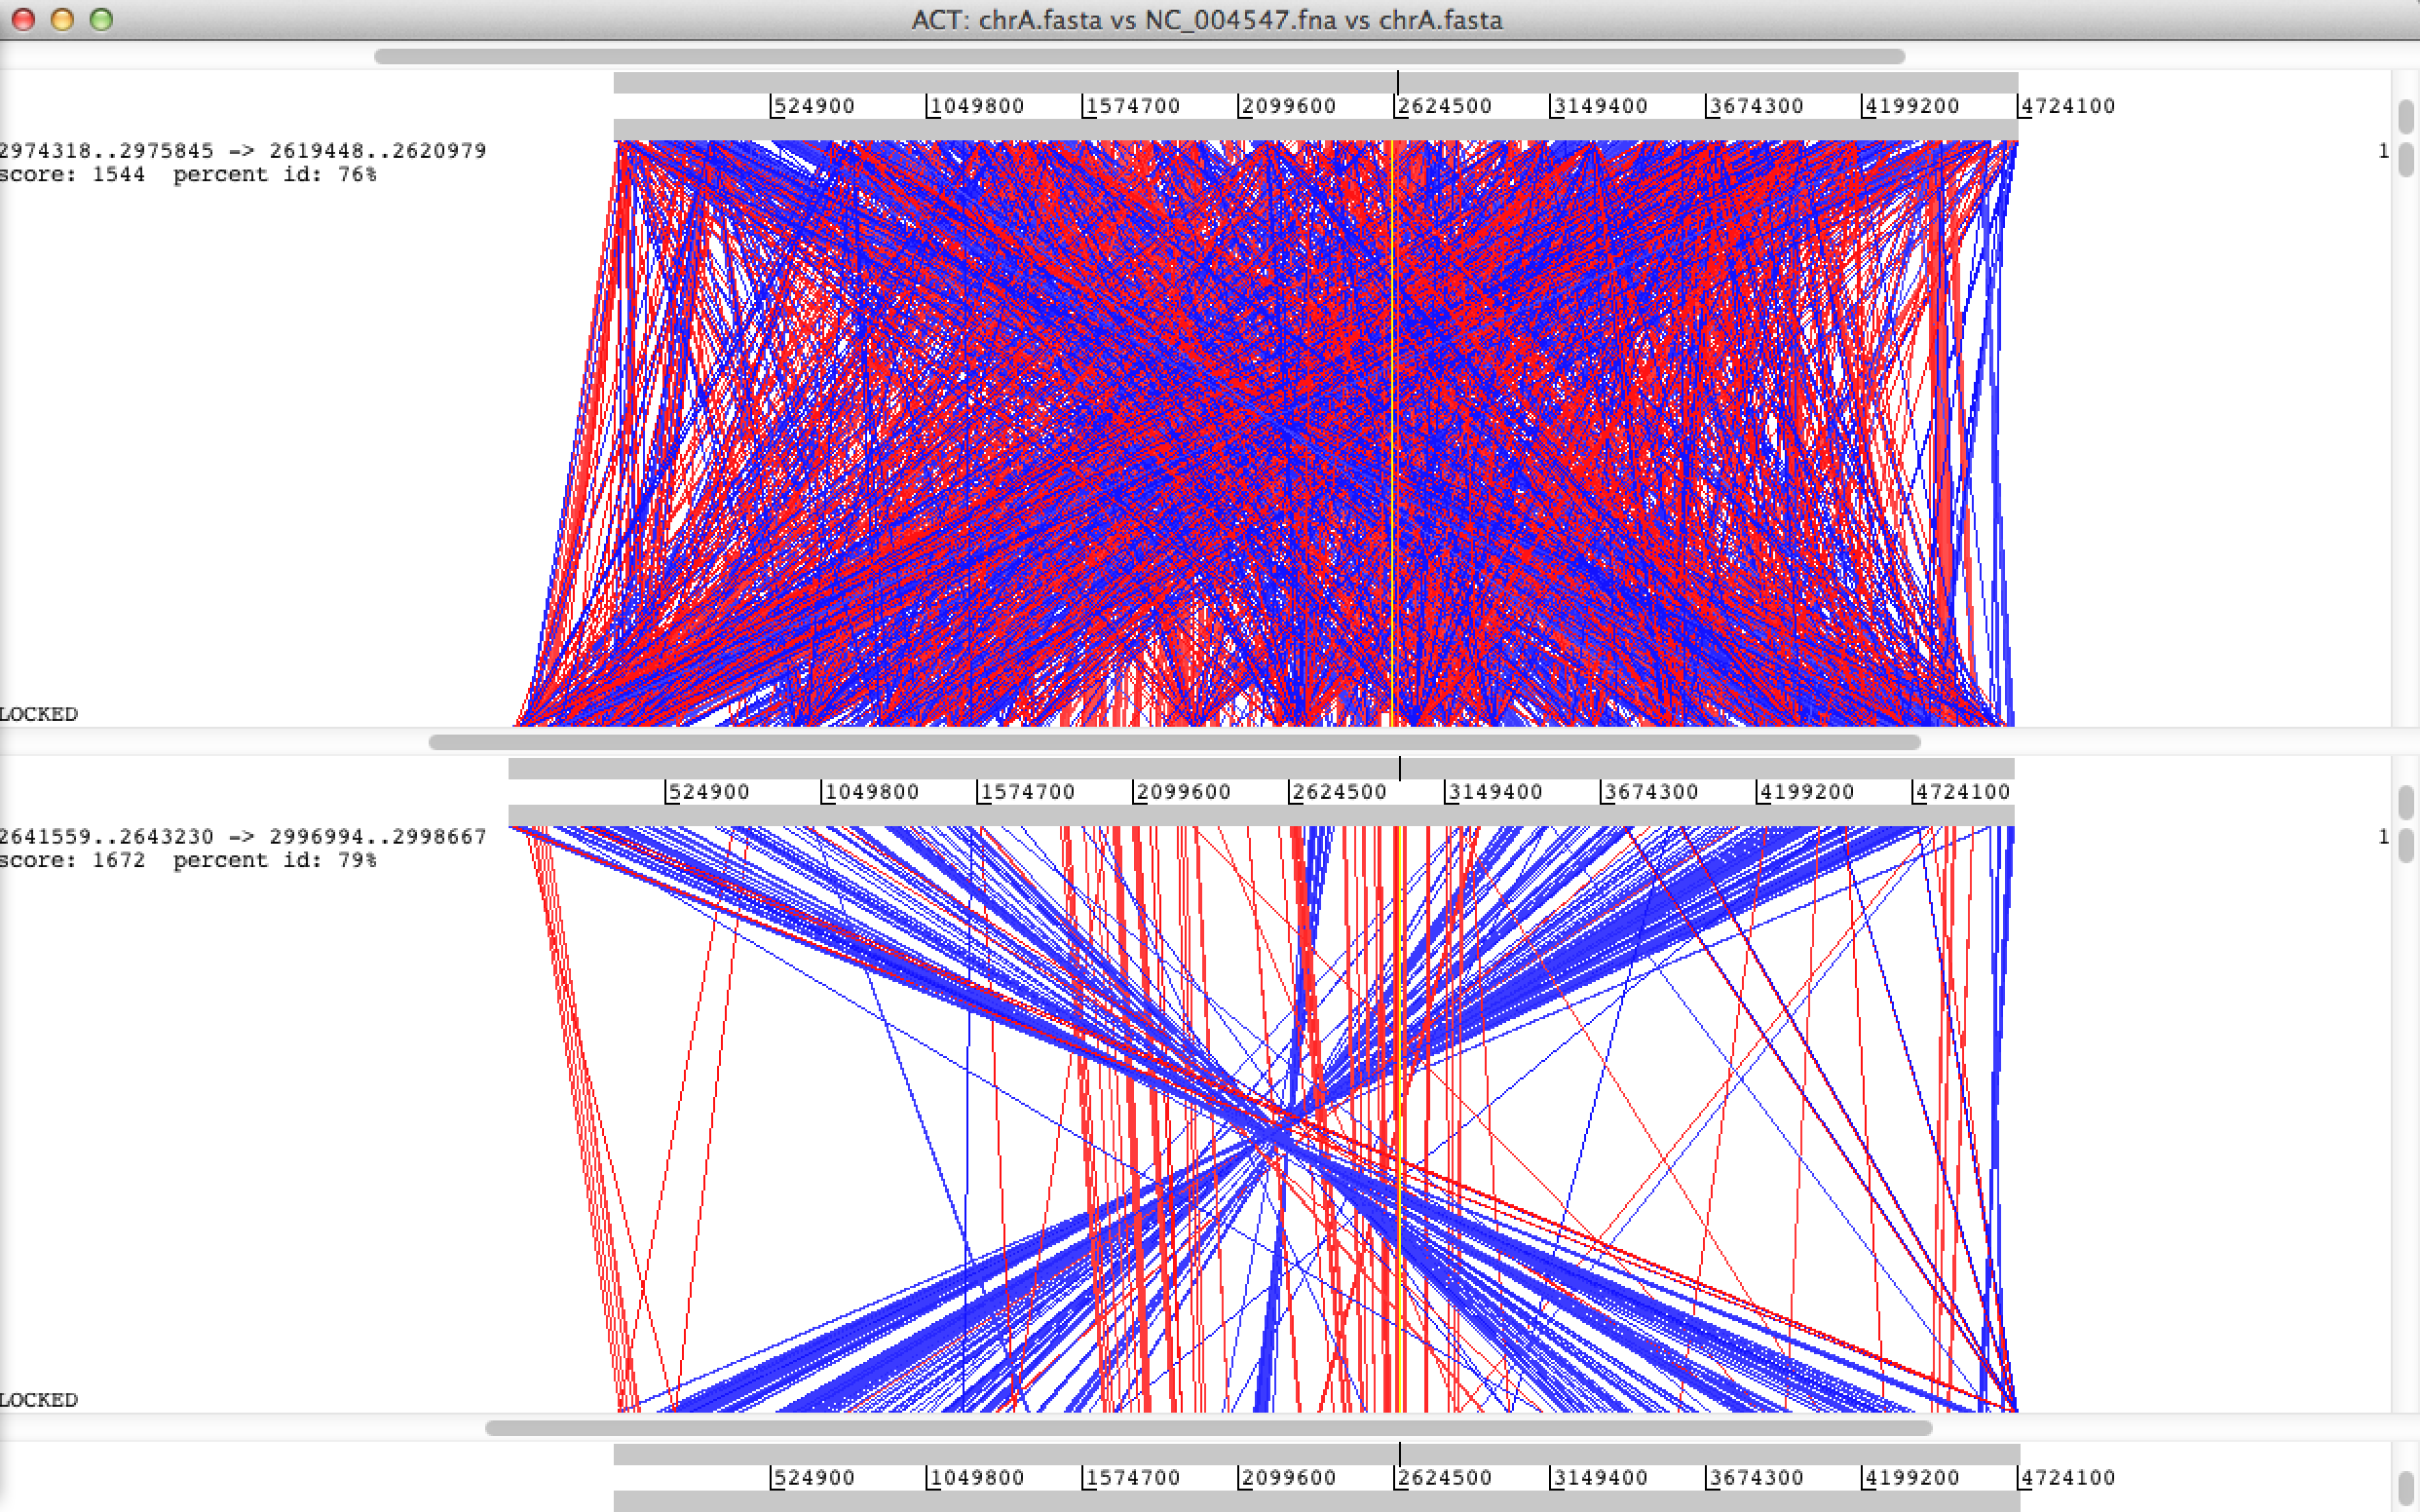
\includegraphics[width=\textwidth]{images/act_rearrangement}
  \end{center}  
\end{frame}

%
\begin{frame}
  \frametitle{Why comparative genomics?}
    \begin{columns}[c] 
      \column{.6\textwidth} 
        \begin{itemize}
         \item \textcolor{hutton_green}{Genome features are heritable characteristics}
         \item \textcolor{hutton_purple}{Related organisms share ancestral genomes}
         \item \textcolor{hutton_blue}{Related organisms inherit common genome features}
         \item \textcolor{RawSienna}{Genome similarity $\propto$ relatedness? (phylogenomics)}
        \end{itemize}
      \column{.4\textwidth}
        
\includegraphics[width=\textwidth]{images/darwin_tree}
    \end{columns}  
\end{frame}

%
\begin{frame}
  \frametitle{Why comparative genomics?}
    \begin{columns}[c] 
      \column{.6\textwidth} 
        \begin{itemize}
         \item \textcolor{hutton_green}{Genomes carry functional elements under selection pressure}
         \item \textcolor{hutton_purple}{Related organisms carry similar functional elements}
         \item \textcolor{hutton_blue}{Deleterious functional elements are lost through selection}         
         \item \textcolor{RawSienna}{Genome similarity $\propto$ phenotype? (functional genomics)}         
        \end{itemize}
      \column{.4\textwidth}
        
\includegraphics[width=\textwidth]{images/darwin_tree}
    \end{columns}  
\end{frame}

%
\begin{frame}
  \frametitle{Why comparative genomics?}
    \begin{columns}[c] 
      \column{.6\textwidth} 
        \begin{itemize}
         \item \textcolor{hutton_green}{Functional elements are selected over many generations}
         \item \textcolor{hutton_purple}{Optimised functional elements may not change greatly}
         \item \textcolor{hutton_blue}{(Functional elements can be transferred non-heritably)}   
         \item \textcolor{RawSienna}{Genome feature similarity $\implies$ common function? (genome annotation)}
         \item \textcolor{red}{Transfer functional information from model systems (\textit{E. coli}, \textit{A. thaliana}, \textit{D. melanogaster}) to non-model systems}
        \end{itemize}
      \column{.4\textwidth}
        
\includegraphics[width=\textwidth]{images/darwin_tree}
    \end{columns}  
\end{frame}

%
\begin{frame}
  \frametitle{Genomes are informative, but$\ldots$}
  \textcolor{hutton_blue}{\textbf{BIOLOGICAL CONTEXT:}} epigenetics, tissue differentiation, mesoscale systems, etc.\\
  \begin{center}  
    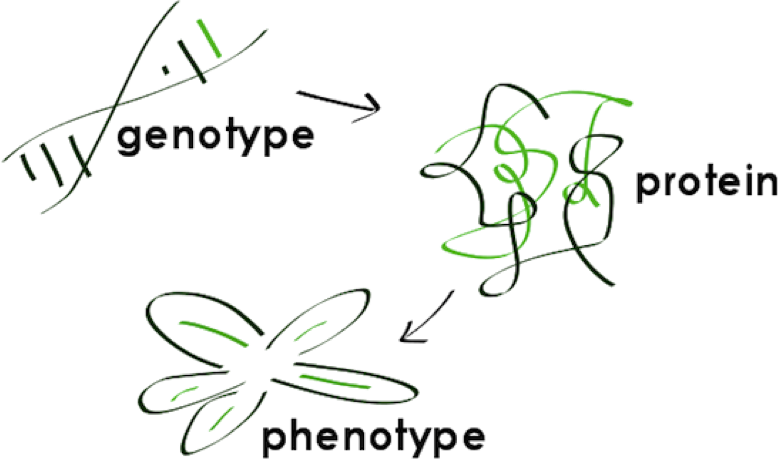
\includegraphics[width=0.7\textwidth]{images/genotype_protein_phenotype}
  \end{center}    
  \textcolor{hutton_green}{\textbf{PHENOTYPIC PLASTICITY:}} responses to temperature, stress, environment, etc.
\end{frame}

%
\begin{frame}
  \frametitle{Genomes to systems}
    \begin{columns}[c] 
      \column{.6\textwidth} 
        \textcolor{RawSienna}{\textbf{Functional Genomics}}
        \begin{itemize}
         \item \textcolor{hutton_green}{Genome differences underpin phenotype (morphological, physiological) differences.}
         \item \textcolor{hutton_purple}{If phenotypes known, genome comparisons can indicate genomic origin of differences (e.g. GWAS).}
         \item \textcolor{hutton_blue}{Genome comparisons can reveal evolutionary processes and constraints, and suggest phenotypic outcomes.}
        \end{itemize}
      \column{.4\textwidth}
        
\includegraphics[width=\textwidth]{images/darwin_tree}
    \end{columns}  
\end{frame}




% SUBSECTION
% Types of genome comparison
\subsection{Types of genome comparison}
%% cladograms.tex
%% Author: Leighton Pritchard
%% Copyright: James Hutton Institute
%% Introductory slides: Cladograms.

%
\begin{frame}
  \frametitle{Types of comparison}
    \begin{columns}[T] 
      \column{.5\textwidth} 
        \textcolor{RawSienna}{\textbf{Within species}}
        \begin{itemize}
	  \item e.g. between isolates/individuals (or between tissues$\ldots$)
	  \item \textcolor{hutton_green}{Which genome features may account for unique characteristics of organisms or cell-types (e.g. tumours)?}
	  \item \textcolor{hutton_blue}{what epigenetic changes occur in an individual?}
	\end{itemize}
      \column{.5\textwidth}
        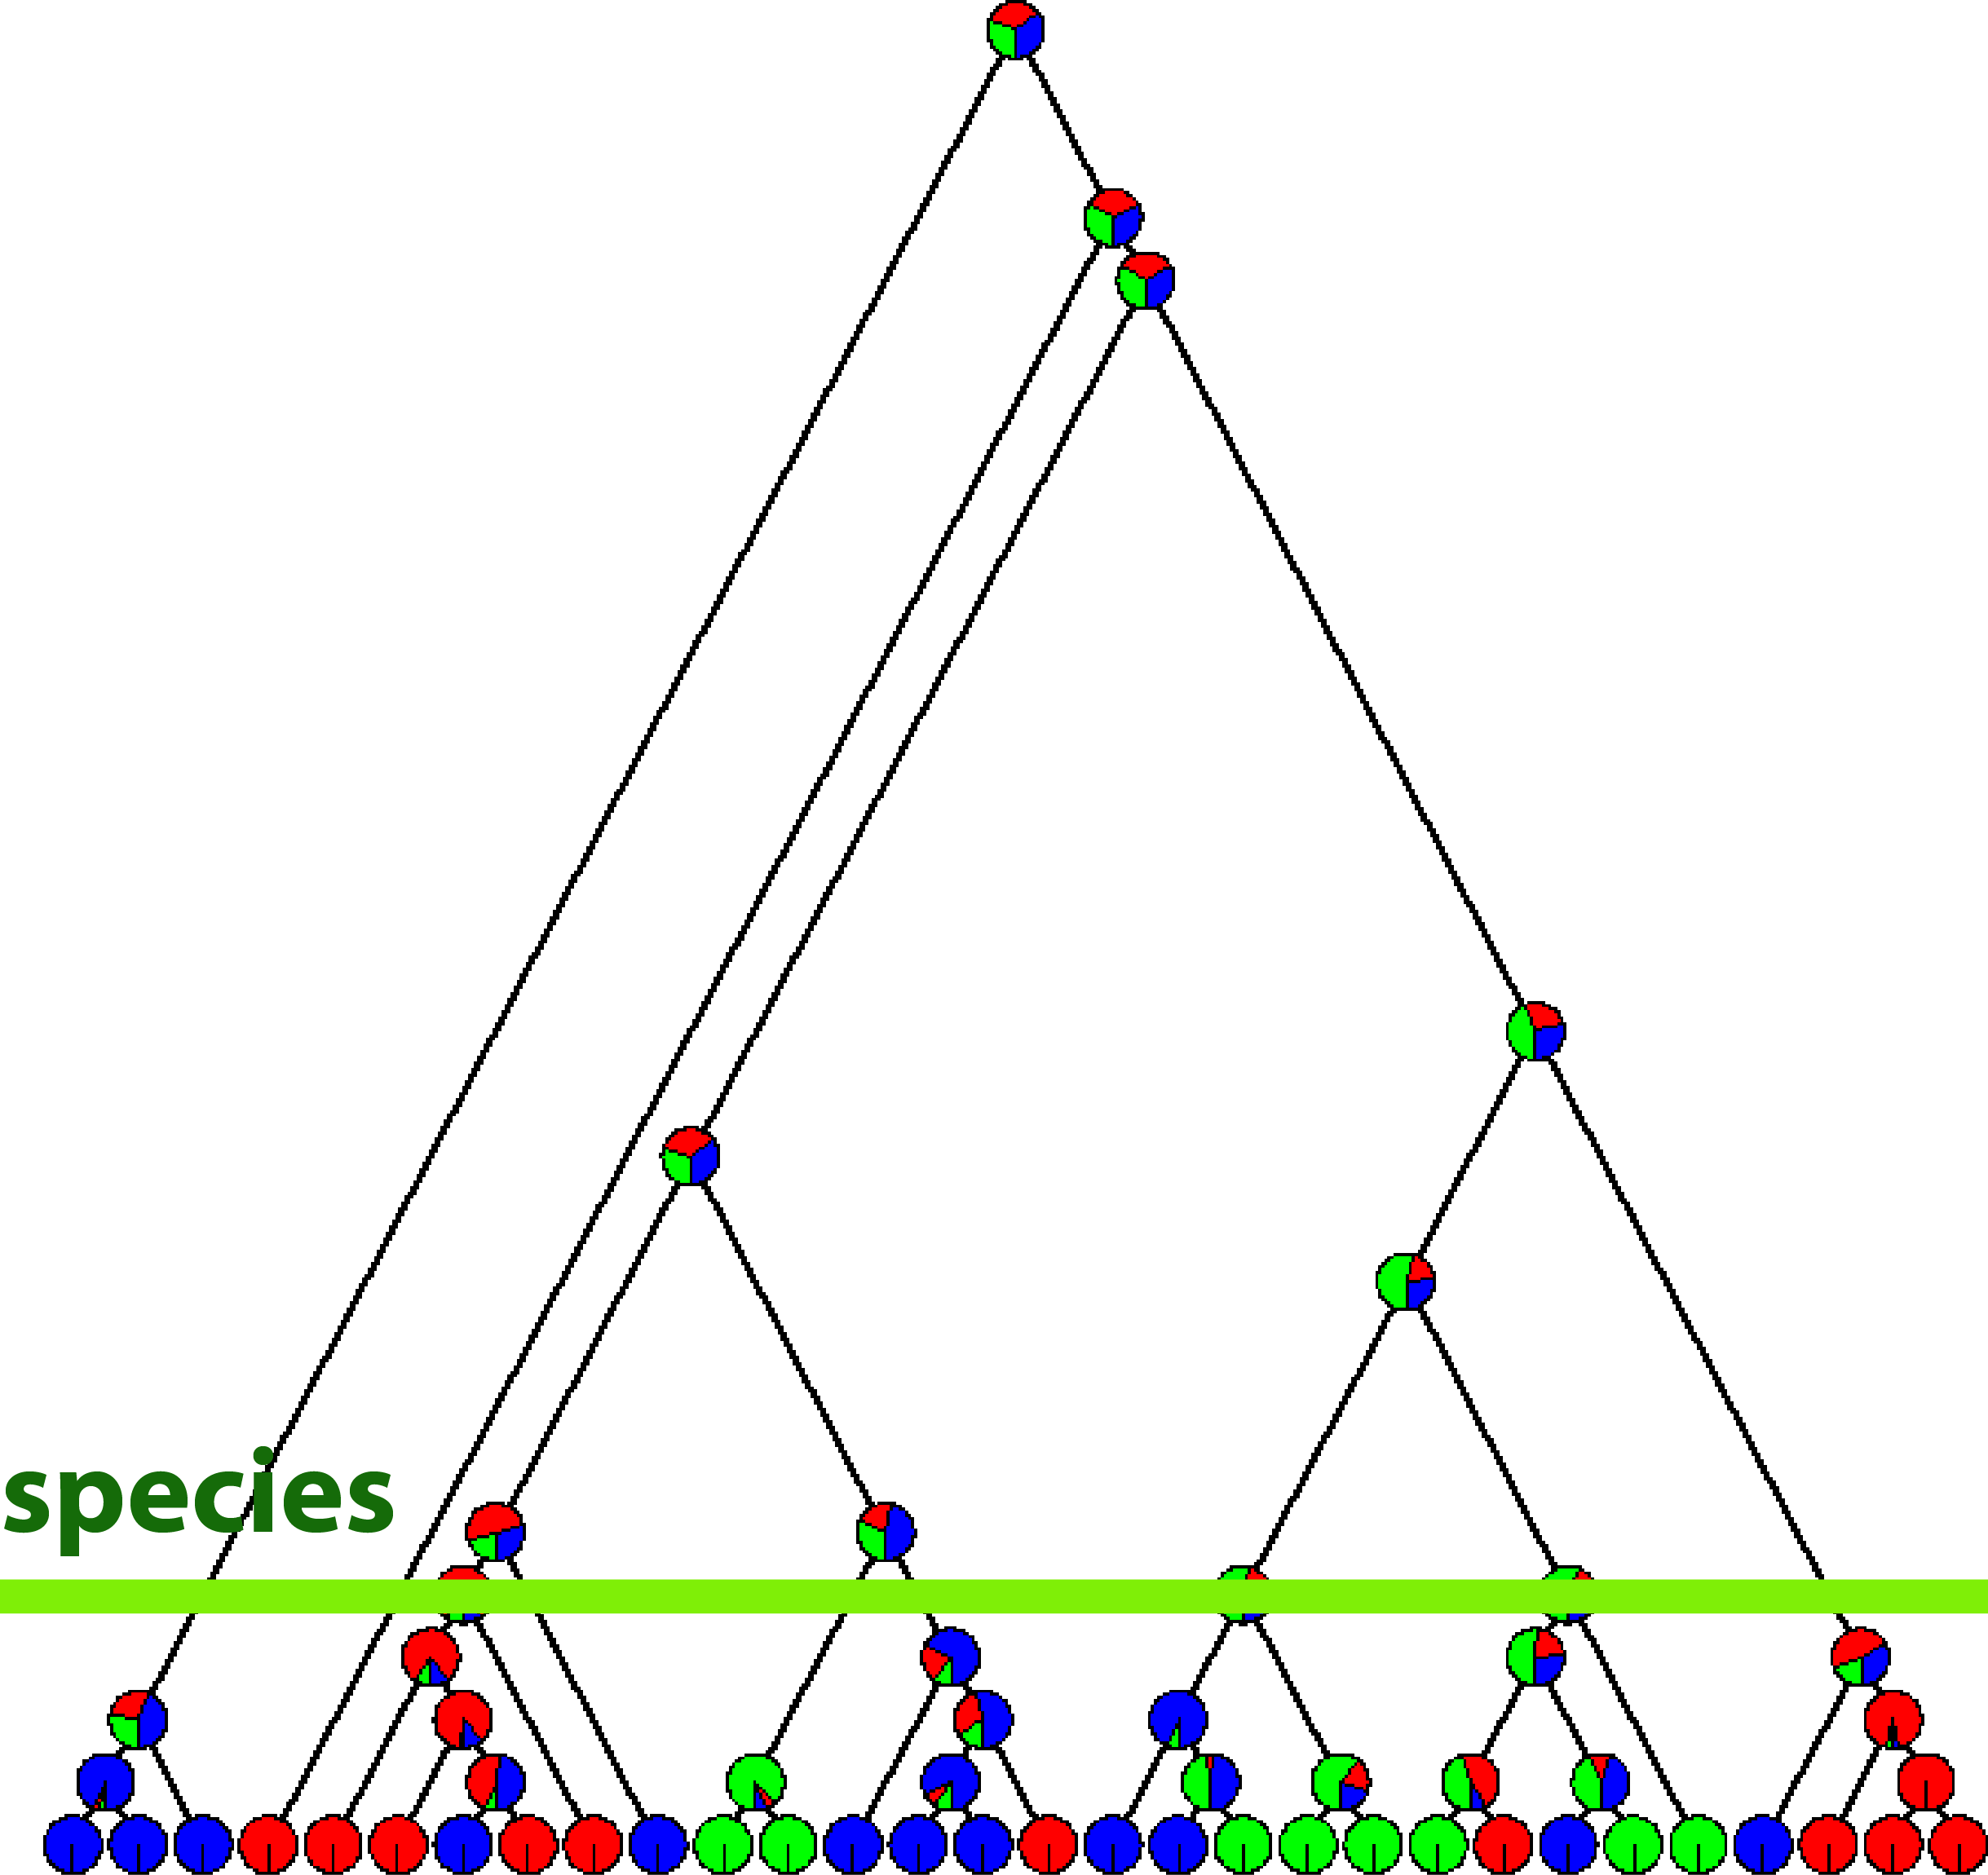
\includegraphics[width=\textwidth]{images/cladogram_species}
    \end{columns}  
\end{frame}

%
\begin{frame}
  \frametitle{Types of comparison}
    \begin{columns}[T] 
      \column{.5\textwidth} 
        \textcolor{RawSienna}{\textbf{Within genera/between species}}
        \begin{itemize}
	  \item comparison between groups of individuals
	  \item \textcolor{hutton_green}{what genome features show evidence of selective pressure?}
	  \item \textcolor{hutton_blue}{which features/changes are associated with species phenotype/adaptation?}      
        \end{itemize}
      \column{.5\textwidth}
        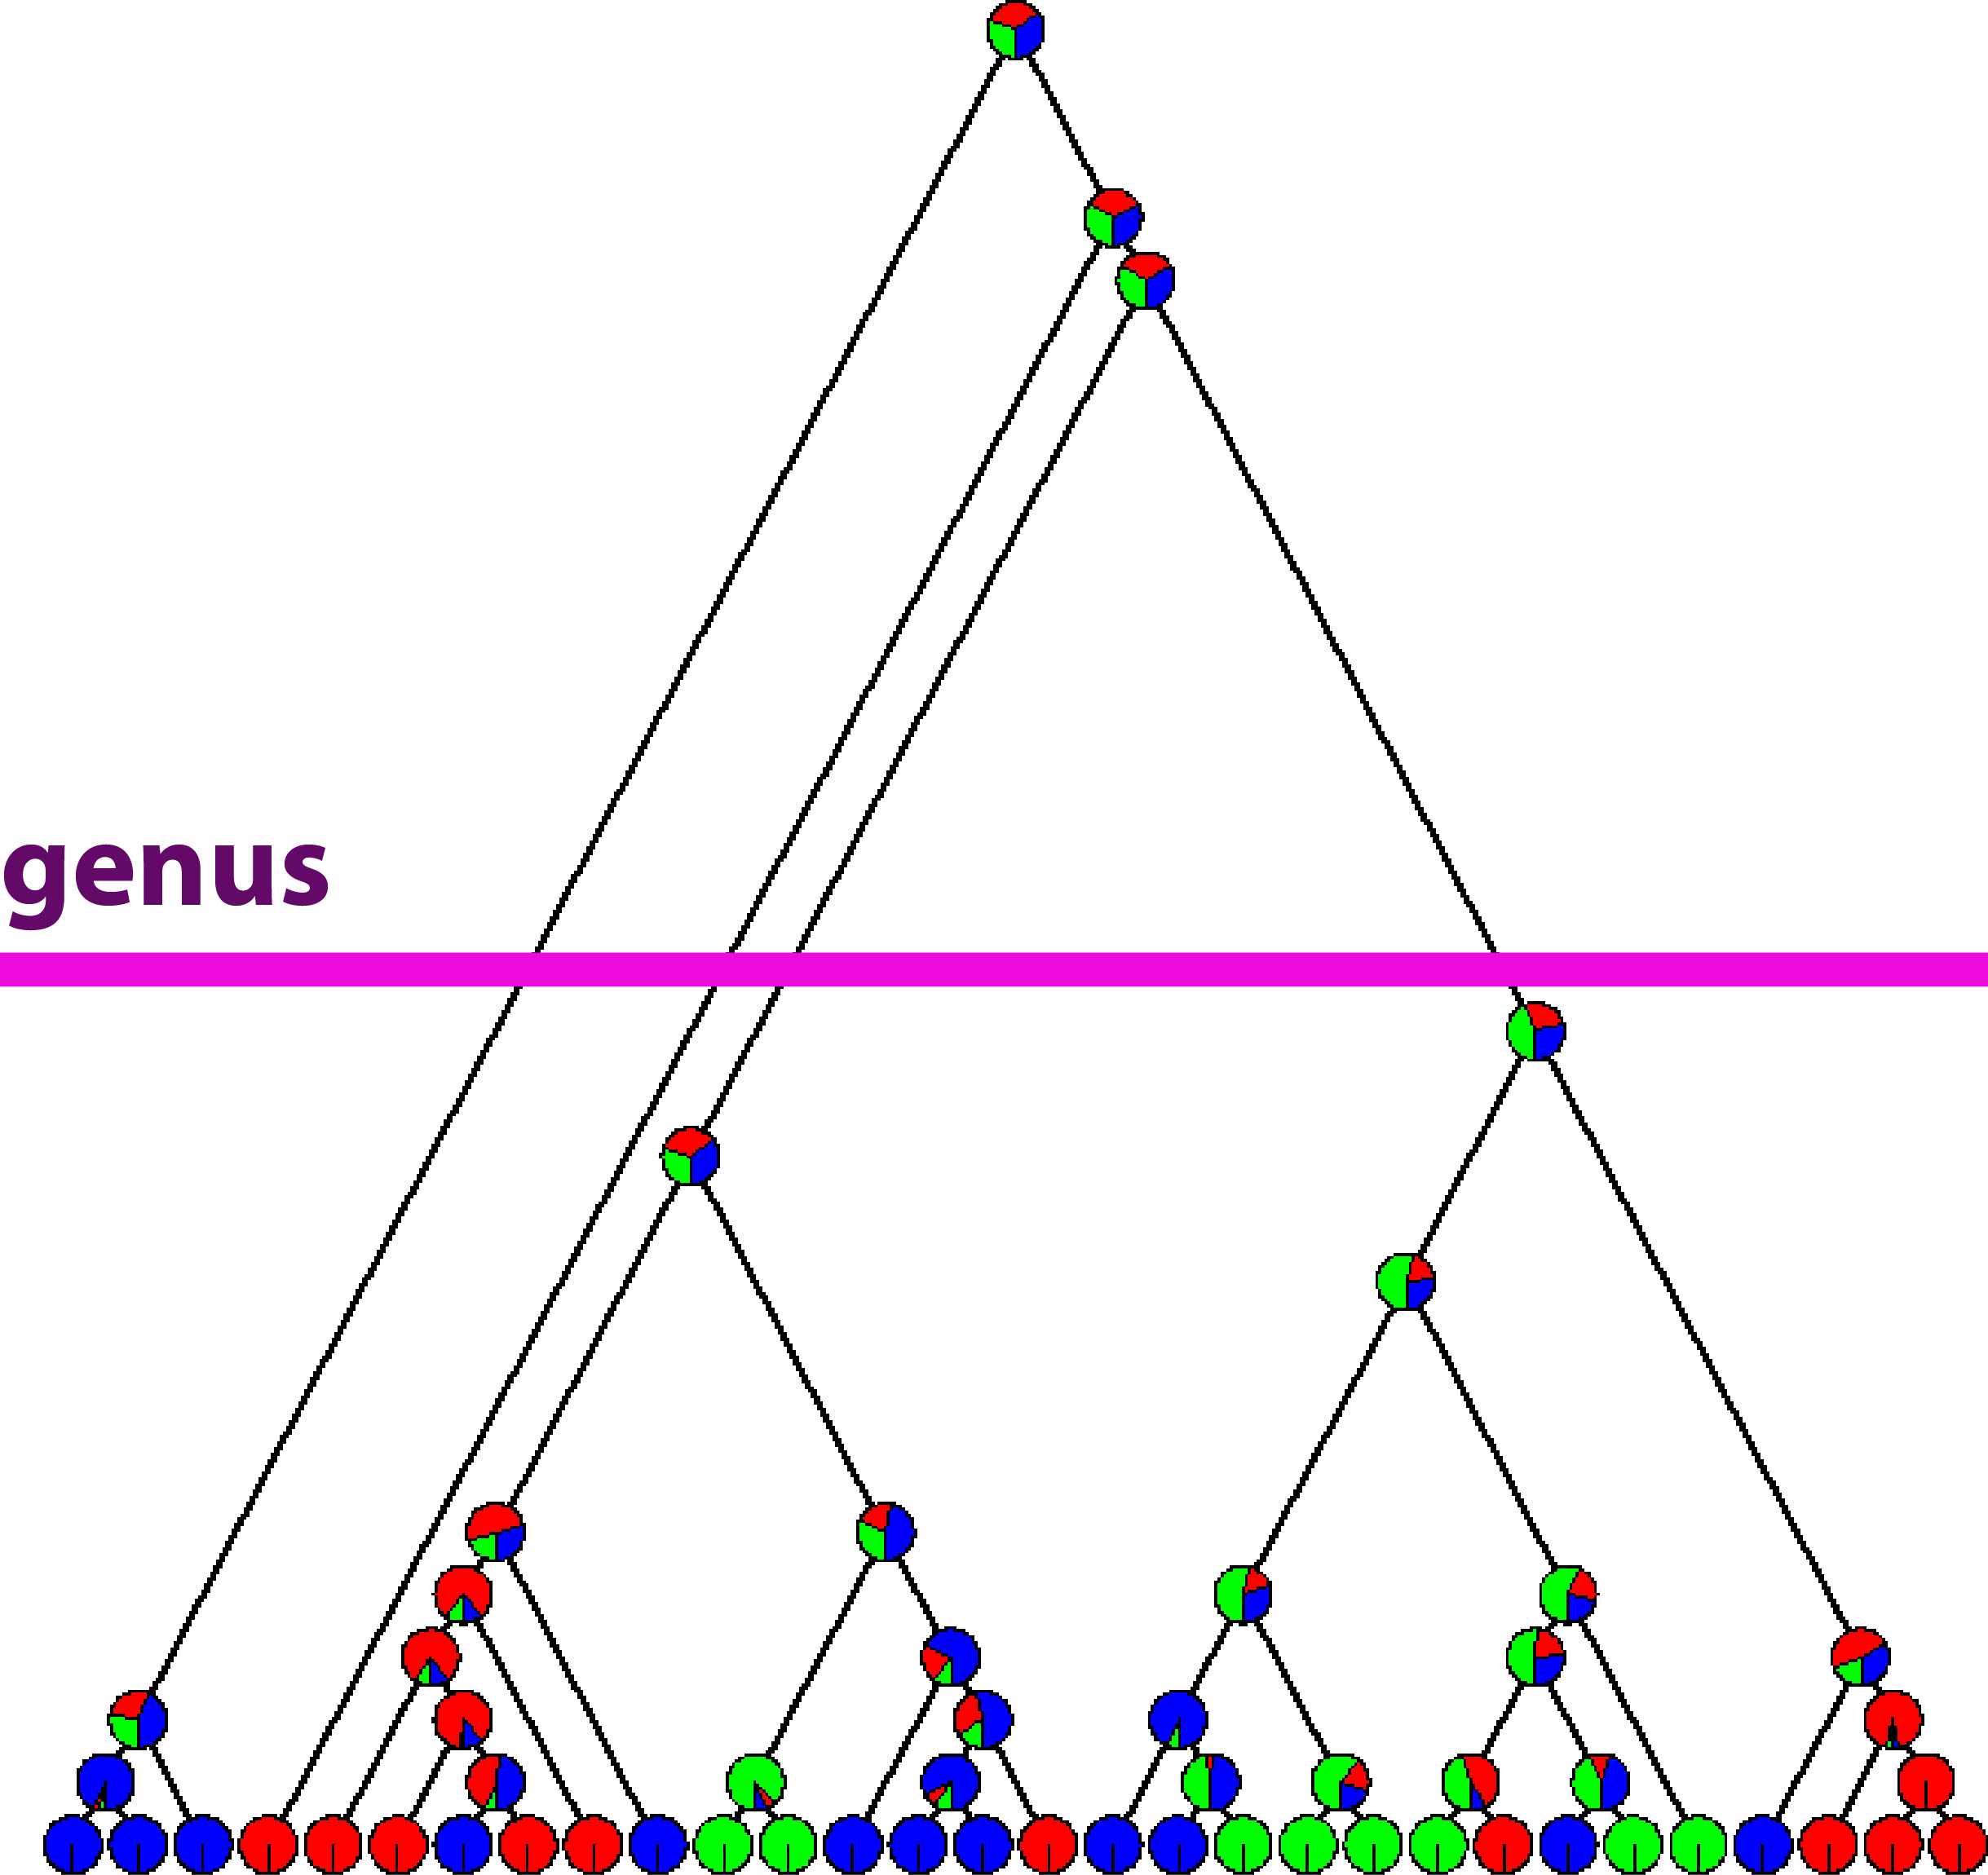
\includegraphics[width=\textwidth]{images/cladogram_genus}
    \end{columns}  
\end{frame}

%
\begin{frame}
  \frametitle{Types of comparison}
    \begin{columns}[T] 
      \column{.5\textwidth} 
        \textcolor{RawSienna}{\textbf{Between subgroups}}
        \begin{itemize}
          \item e.g. comparisons across many diverse individuals
          \item \textcolor{hutton_green}{what are the \textit{core set} of genome features that define a subgroup or genus?}
          \item \textcolor{hutton_blue}{what functions are present/absent between groups?}
        \end{itemize}
      \column{.5\textwidth}
        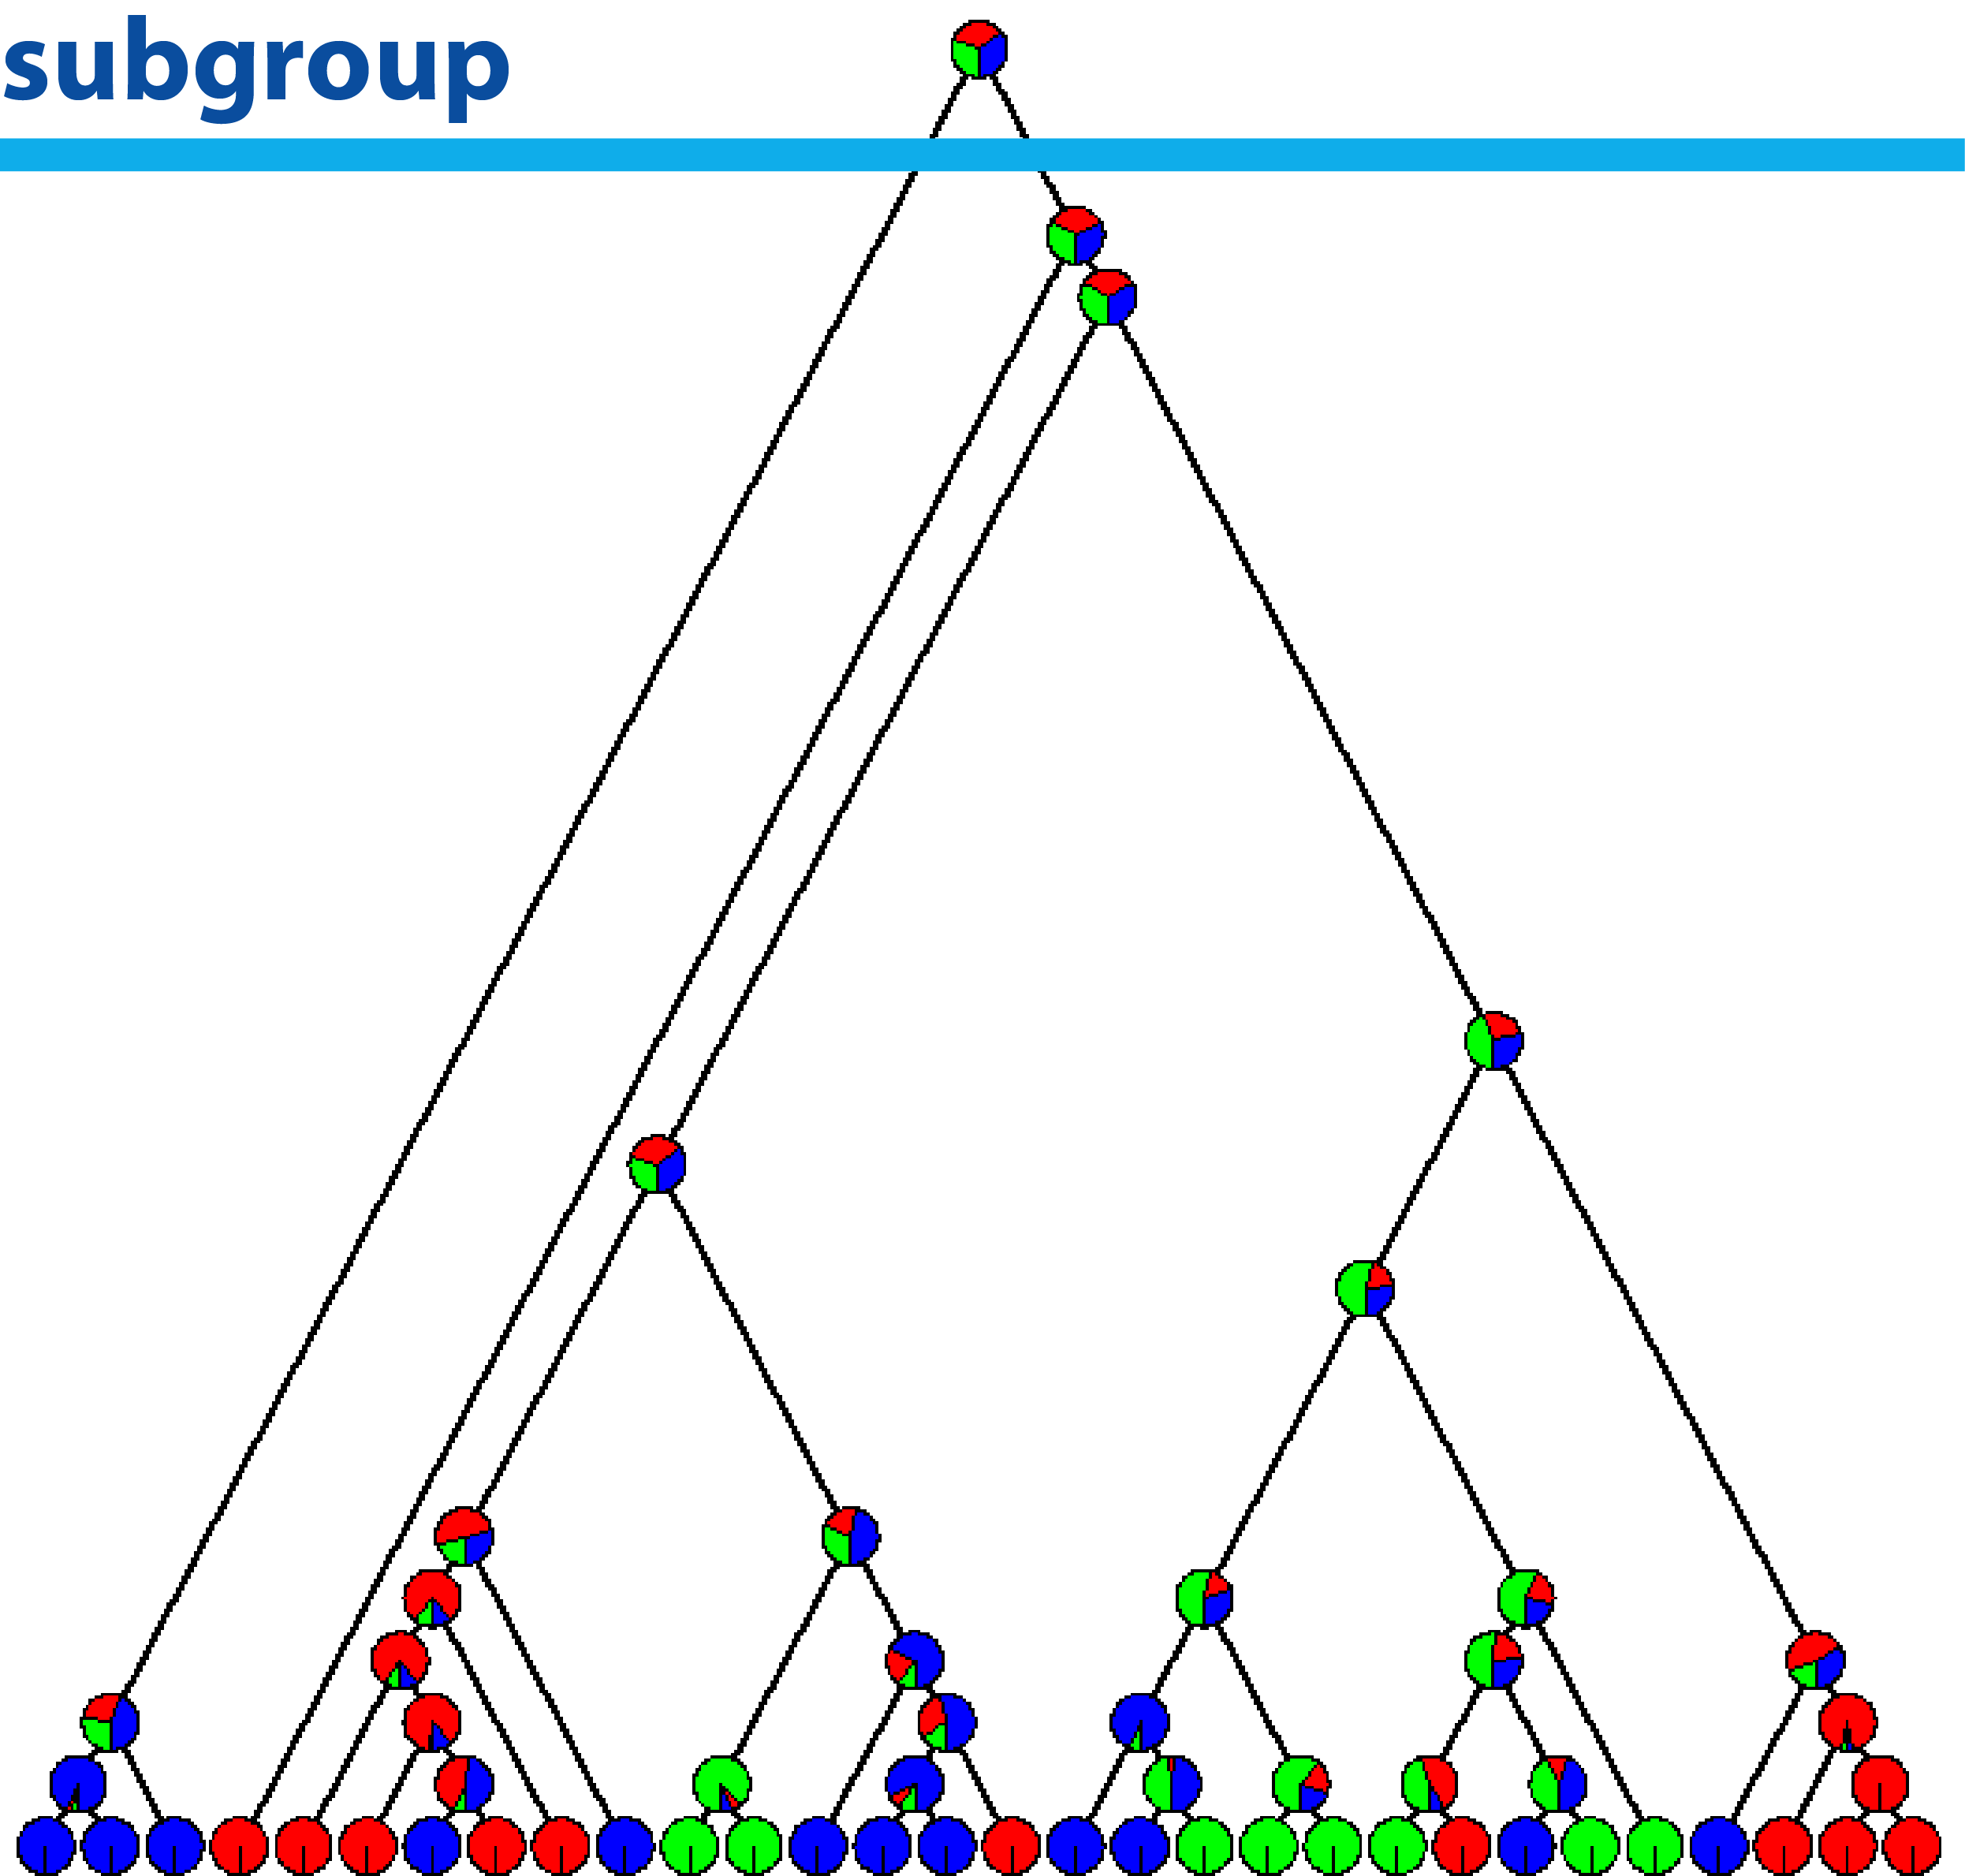
\includegraphics[width=\textwidth]{images/cladogram_subgroup}
    \end{columns}  
\end{frame}
%% ltee.tex
%% Author: Leighton Pritchard
%% Copyright: James Hutton Institute
%% Example slides: The Long-Term Evolution Experiment

%
\begin{frame}
  \frametitle{\textit{E. coli} LTEE
                   \footnote{\tiny{\href{http://dx.doi.org/10.1016/j.jmb.2009.09.052
}{Jeong \textit{et al}. (2009) \textit{J. Mol. Biol.} doi:10.1016/j.jmb.2009.09.052
}}}
                   \footnote{\tiny{\href{http://dx.doi.org/10.1038/nature08480
}{Barrick \textit{et al}. (2009) \textit{Nature} doi:10.1038/nature08480
}}}
                   \footnote{\tiny{\href{http://dx.doi.org/10.1126/science.1243357
}{Wiser \textit{et al}. (2013) \textit{Science} doi:10.1126/science.1243357
}}}}
    \begin{columns}[c] 
      \column{.6\textwidth} 
        \begin{itemize}
          \item \textcolor{RawSienna}{Run by the Lenski lab, Michigan State University since 1988 \\
          (\href{http://myxo.css.msu.edu/ecoli/}{http://myxo.css.msu.edu/ecoli/})}
          \item \textcolor{hutton_green}{12 flasks, citrate usage selection}
          \item \textcolor{hutton_blue}{$>$50,000 generations of \textit{E coli}!}
          \begin{itemize}
            \item Cultures propagated every day
            \item Every 500 generations (75 days), mixed-population samples stored
            \item Mean fitness estimated at 500 generation intervals
          \end{itemize}
        \end{itemize}
      \column{.4\textwidth}
        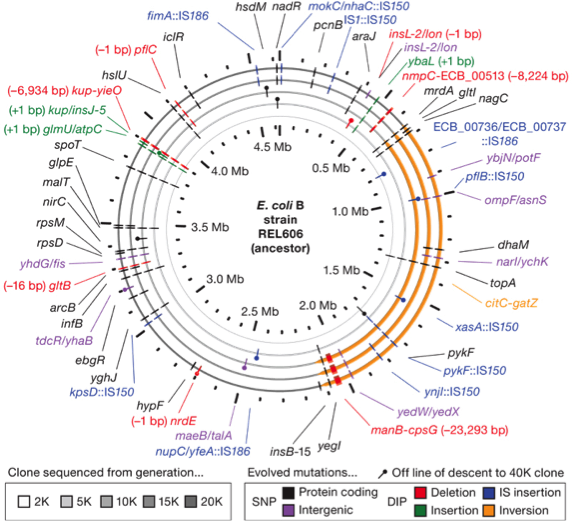
\includegraphics[width=\textwidth]{images/ltee_circular} \\
        
\includegraphics[width=\textwidth]{images/ltee_linear}        
    \end{columns}  
\end{frame}
%% utricularia.tex
%% Author: Leighton Pritchard
%% Copyright: James Hutton Institute
%% Example slides: Comparative Genomics In The News 2015

%
\begin{frame}
  \frametitle{Comparative genomics in the news
                   \footnote{\tiny{\href{http://www.washingtonpost.com/news/speaking-of-science/wp/2015/02/23/the-mysterious-genes-of-carnivorous-bladderwort-reveal-themselves/
}{Washington Post 23/2/2015
}}}
                   \footnote{\tiny{\href{http://dx.doi.org/10.1038/nature12132
}{Ibarra-Laclette \textit{et al}. (2013) \textit{Nature} doi:10.1038/nature12132
}}}
                   \footnote{\tiny{\href{http://dx.doi.org/10.1093/molbev/msv020
}{Carretero-Paulet \textit{et al}. (2015) \textit{Mol. Biol. Evol.} doi:10.1093/molbev/msv020
}}}
}
    \begin{columns}[c] 
      \column{.6\textwidth} 
        \begin{itemize}
          \item \textcolor{RawSienna}{\textit{Utricularia gibba}: carnivorous bladderwort}
          \item \textcolor{hutton_blue}{Genome: 82Mbp, 17,324 genes \\
          (wheat: 17bn bases, $\approx$94-96k genes)}
          \item Intergenic region contraction \\
          (3\% repeat elements; most plants: 10-60\% repeat elements)
          \item \textcolor{hutton_green}{Genomic context for flowering plants does not require ``hidden regulators'' (cf. ENCODE)}
        \end{itemize}
      \column{.4\textwidth}
        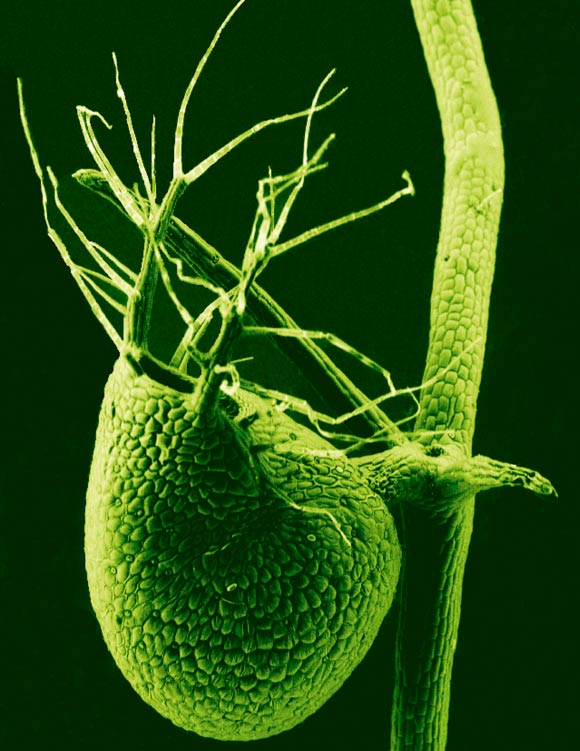
\includegraphics[height=0.3\textheight]{images/Utricularia-gibba}
        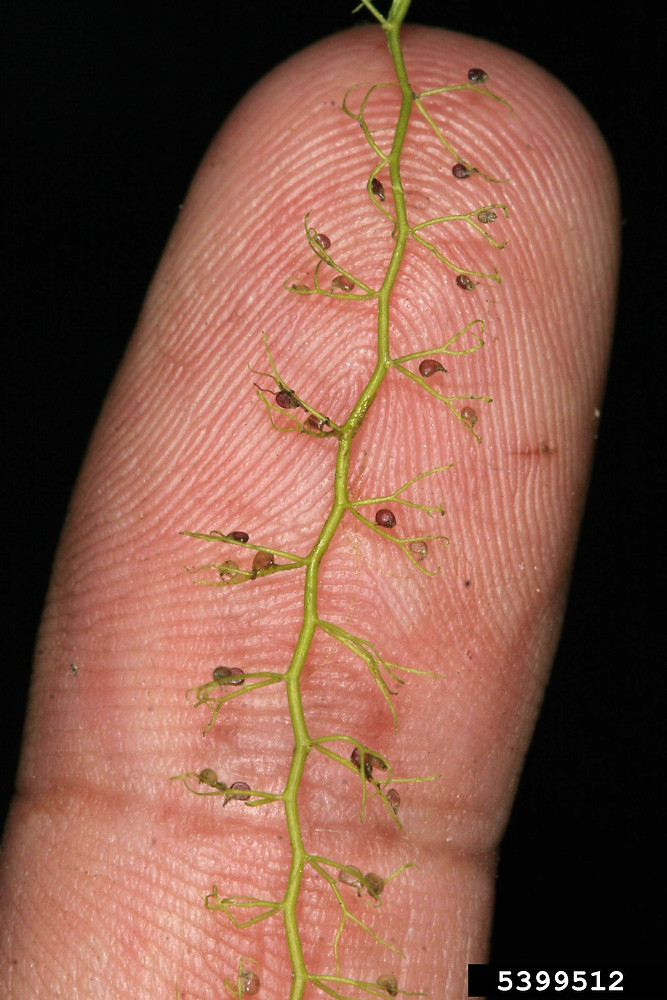
\includegraphics[height=0.3\textheight]{images/utricularia-gibba-finger} \\
        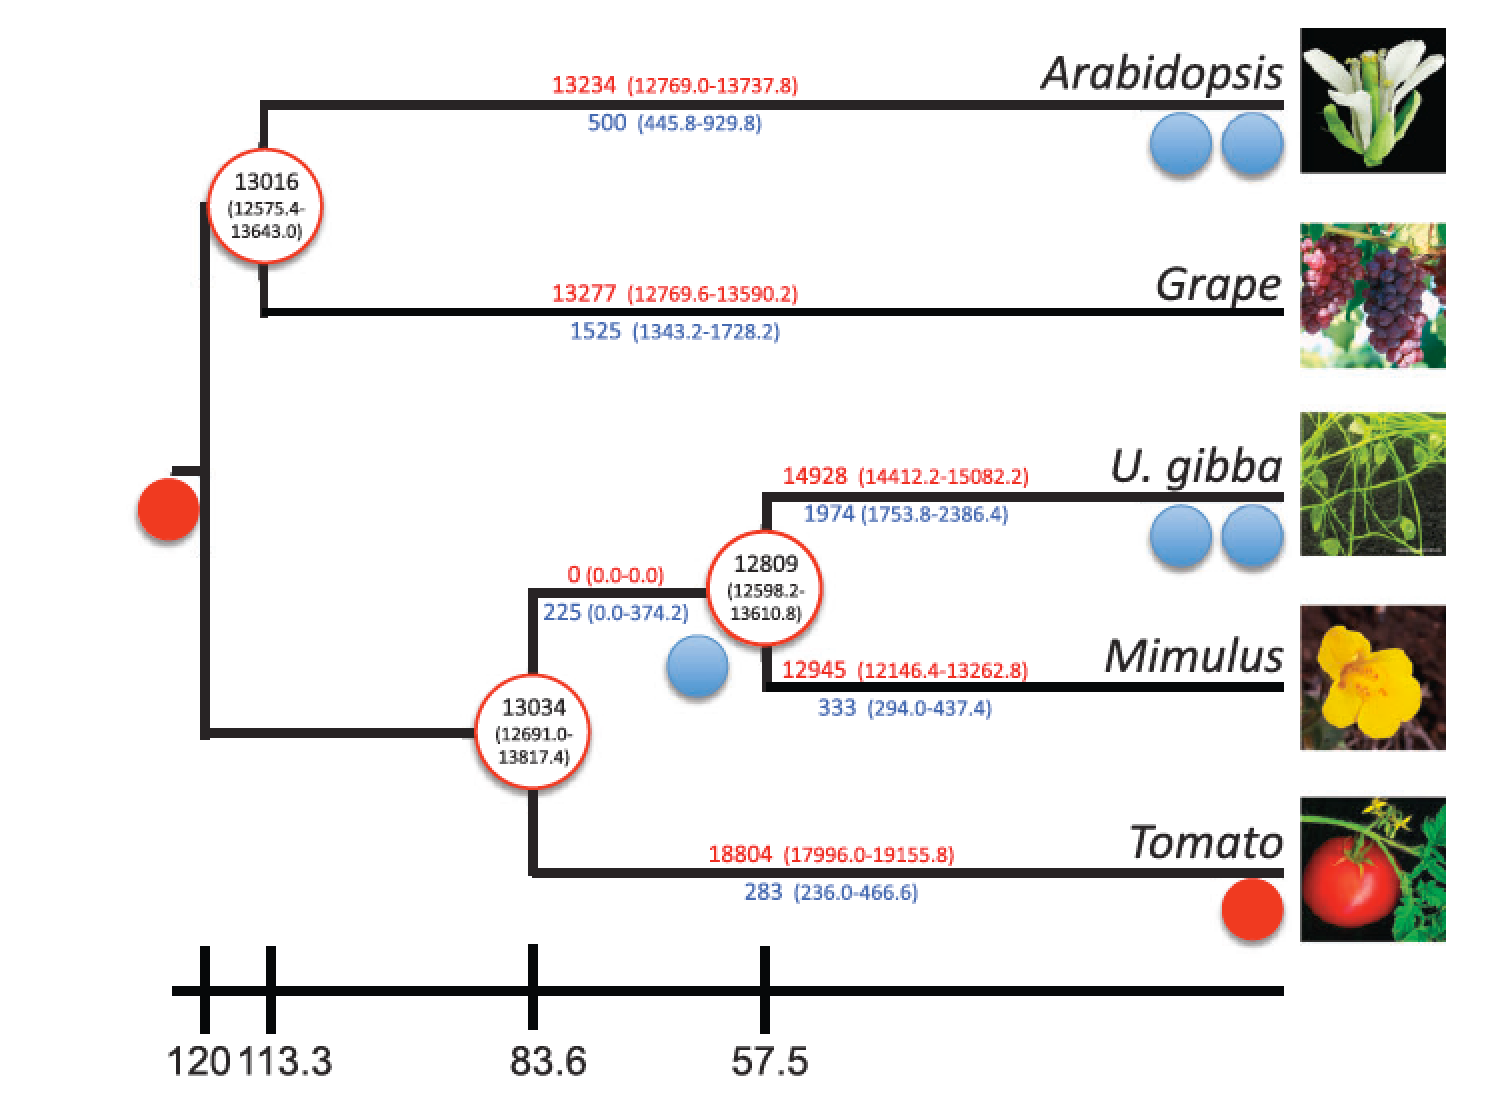
\includegraphics[width=\textwidth]{images/U_gibba_tree}        
    \end{columns}  
\end{frame}
%% mcq1.tex
%% Author: Leighton Pritchard
%% Copyright: James Hutton Institute
%% This slide offers a multiple choice question.

%
\begin{frame}
  \frametitle{Question:}
  \textbf{Which of these questions can be answered by comparative genomics?}
  \begin{itemize}
    \item A: Are genes in a metabolic pathway always collocated?
    \item B: What genes does a transcription factor regulate?
    \item C: Which genes in a genome are under positive selective pressure?
    \item D: What genome features can be used to define a species?
  \end{itemize}
\end{frame}
% SUBSECTION
% Course outline
\subsection{Course outline}
%% comparison_types.tex
%% Author: Leighton Pritchard
%% Copyright: James Hutton Institute
%% Introductory slides: Types of comparison

%
\begin{frame}
  \frametitle{Levels of comparison}
  \textbf{Bulk Properties} \\
  \begin{itemize}  
    \item \textcolor{hutton_green}{chromosome/plasmid counts and sizes, nucleotide content, etc.}
  \end{itemize}    
  \textbf{Whole Genome Sequence} \\
    \begin{itemize}
      \item \textcolor{hutton_blue}{sequence similarity}
      \item \textcolor{hutton_blue}{organisation of genomic regions (synteny), etc.}
    \end{itemize}
  \textbf{Genome Features/Functional Components} \\
  \begin{itemize}
    \item \textcolor{hutton_purple}{numbers and types of features (genes, ncRNA, regulatory elements, etc.)}
    \item \textcolor{hutton_purple}{organisation of features (synteny, operons, regulons, etc.)}
    \item \textcolor{hutton_purple}{complements of features}
    \item \textcolor{hutton_purple}{selection pressure, etc.}
  \end{itemize}
\end{frame}


%%%
% LICENCE FOR REUSE
%% licence.tex
%% Author: Leighton Pritchard
%% Copyright: James Hutton Institute
%% These slides describe the licence for reuse of these slides and
%% materials

%
\begin{frame}
  \frametitle{Licence: CC-BY-SA}
  By: Leighton Pritchard \\[0.5cm]
  This presentation is licensed under the Creative Commons Attribution ShareAlike license \\
  \href{https://creativecommons.org/licenses/by-sa/4.0/}{https://creativecommons.org/licenses/by-sa/4.0/}
\end{frame}

% etc
\end{document}